\subsection*{Goal}
  \frame{\frametitle{Change point detection context}
    \begin{tabular}{p{0.5\textwidth} p{0.4\textwidth}}
    \begin{tabular}{p{\textwidth}}
        \includegraphics<1>[height=.6\textheight]{rawSignal}
        \includegraphics<2>[height=.6\textheight]{segmentedSignal}
      \end{tabular}
    &  
      \begin{tabular}{p{0.4\textwidth}}
        \onslide<1>{ \emph{Goal : } Identifying homogenous regions and abrupt changes in the signal.\\}
        \onslide<2>{ These \textcolor{red}{regions} may be interpreted afterwards.\\}
    \end{tabular}
  \end{tabular}
  }


\subsection*{Model}
\begin{frame}{Underlying model}


\only<1>{ Modelling~:}
\only<2>{\textcolor{red}{Change point detection in the trend (and/or in variance)~:} }
    \begin{itemize}
    \item Data $Y_1,\ldots,Y_n$ are drawn from a given pdf, driven by unknown parameter $\theta$
      \begin{equation*}
        Y_i \overset{i.i.d}{\sim} f_{\theta}(.)  \ \ 
      \end{equation*}
     $\theta$ values change at  $K-1$ unknow instants, the change point~:
     $t_1,\ldots,t_{K-1}$ :
     \only<1>{\begin{equation*}
         Y_t \sim f(\theta_k) \ \ \mbox{if $t$ in region $I_k=[t_{k-1}+1,t_{k}]$}
        \end{equation*}}
       \only<2->{ \textcolor{red}{
           \begin{equation*}
             Y_t\overset{ind}{\sim} \Ncal(\mu_k,\sigma^2) 
             \mbox{ if $t$ in portion $I_k$,  for  $k=1,\ldots,K$. }
           \end{equation*}
       } }
       \end{itemize}

  

 \onslide<3->{
  \begin{columns}
  \begin{column}{0.7\textwidth}
   \includegraphics[scale=0.3]{segCode1-1.pdf}
   \end{column}
   \begin{column}{0.3\textwidth}
  \noindent Remark : $K-1$ change points  $\Leftrightarrow$ $K$ regions.
   \end{column}
   \end{columns}
  }
\end{frame}

 
 \subsection*{Estimation}
 \frame{\frametitle{Estimation procedure}
   \begin{itemize}
   \item Unknown parameters : $\mubf=(\mu_1, \ldots, \mu_{\textcolor{red}{K}})$, $\sigma$, and $\Tbf=(T_1, \ldots, T_{\textcolor{red}{K}})$,\\
     but  also \textcolor{red}{K} itself.
   \onslide<3->{
   \item Estimation Procedure
   \only<3->{
    \begin{itemize}}
    \only<3>{
       \item For  given $K$ and $\Tbf$,   $\thetabf$ is estimated using maximum likelihood.}
       \only<4>{\item For  given $K$, compute the maximum likelihood for any possible position for $\Tbf$, 
       \textcolor{red}{But, } $$\left( \begin{array}{c} n-1 \\ K-1 \end{array}\right)$$ possible choices for the $K-1$ positions, that is $10^{30}$ for $K=10$, $n=200$,  ( $\approx 10^{11}$ years on a 2014 computer).
       \pause
  \centerline{$\Rightarrow$ Practically impossible even for small $K$ and $n$}
  \centerline{\textcolor{red}{Dynamic programming}}
       }
  \only<5>{
  \item Estimating $K$. 
     Likelihood increases with the number of segment $K$, use a penalized likelihood criterion and
    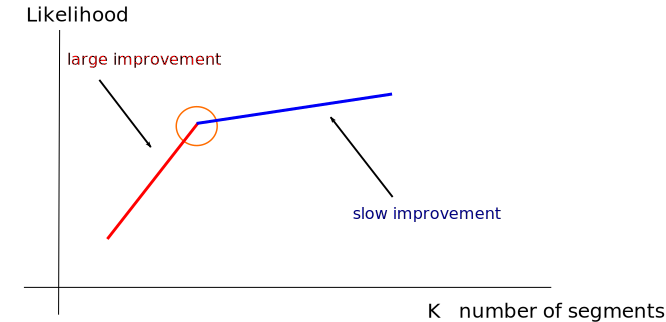
\includegraphics[scale=0.3]{LikelihoodProfile}
  }
  \only<3->{\end{itemize}}
   }
\end{itemize} 
}


\frame{\frametitle{Estimation procedure}

\paragraph{Likelihood}
{\small
\begin{eqnarray*}
2 log(P_K (\Ybf, \Tbf, \thetabf)) & = & 2 \sum_{k=1}^K \log f(\{Y_t\}_{t \in
I_k};
\theta_k) = 2 \sum_{k=1}^K \sum_{t \in I_k}\log f(Y_t; \theta_k) \\
& = & -n \log \sigma^2 - \frac1{\sigma^2} \sum_{k=1}^K \sum_{t \in
  I_k} (Y_t - \mu_k)^2 + \mbox{cst}.
\end{eqnarray*}
}

\paragraph{Estimations}
\begin{equation*}
 (\hat{\Tbf},\hat{\thetabf})=
  \argmax_{(\Tbf,\thetabf)} log(P_K (\Ybf, \Tbf, \thetabf))
\end{equation*}

\paragraph{If the change points are known}
\begin{columns}
\begin{column}{0.5\textwidth}
\begin{equation*}
\widehat{\mu}_k = \frac1{n_k} \sum_{t \in I_k} Y_t
\end{equation*}
\end{column}
\begin{column}{0.5\textwidth}
  $$
  \widehat{\sigma}^2 =  \frac1{n} \sum_{k=1}^K \sum_{t \in I_k} (Y_t -  \widehat{\mu}_k)^2
  $$
\end{column}
\end{columns}
}
% 
\begin{frame}[fragile]{Finding the K-1 change points}
 \only<1-3>{
 \paragraph{Considering all possible segmentations, } the best segmentation minimizes 
 $$
 J_k(1, n) = \sum_{k=1}^K \sum_{t \in I_k} (Y_t - \widehat{\mu}_k)^2.
 $$
 \pause
 \paragraph{Dynamic programming,} with complexity ($\mathcal{O}(n^2)$).
 } 
 
% %possible only because the quantity of interest is the sum over all segments 
% 
% %%%%%%%%%%%%%%%%%%%%%%%%%%%%%%%%%%%%%%%%%%%%%%%%%%%%%%%%%%%%%%%%%%%%%%
% %%%%%%%%%%%%%%%%%%%%%%%%%%%%%%%%%%%%%%%%%%%%%%%%%%%%%%%%%%%%%%%%%%%%%%
 \only<4>{\centerline{\sl Sub-paths of the optimal path are themselves
 optimal,} 
 Bellmann optimality 
 $$ $$
 \begin{description}
% 
 \item[Initialisation:] Compute for $0 \leq i < j \leq n$, cost of portion $I_{ij}$~:
  $$
  J_1(i, j) = \sum_{t=i+1}^j (Y_t - \widehat{\mu})^2
  $$
 \item[Etape $k$:] Compute for $2 \leq k \leq K$, $J_k(i, j)$ the cost of the best segmentation in $k$ segments between $i$ and $j$.
   $$
   J_k(i, j) = \min_{i < h <j} \left[J_{k-1}(i, h) + J_1(h+1,  j)\right].
   $$
 \end{description}
 }
\end{frame}

% 
\subsection*{Example}
\subsection*{ Toy Example}
   \begin{frame}[fragile]{How to perform this segmentation approach ?}
 
\begin{columns}
\begin{column}{0.4\textwidth}
\begin{knitrout}
\definecolor{shadecolor}{rgb}{0.969, 0.969, 0.969}\color{fgcolor}\begin{kframe}
\begin{alltt}
\hlkwd{load}\hlstd{(}\hlstr{"../Data/dataSegmentation.Rd"}\hlstd{)}
\hlkwd{summary}\hlstd{(Profil.seg)}
\end{alltt}
\begin{verbatim}
##    Min. 1st Qu.  Median    Mean 3rd Qu.    Max. 
##  0.8904  4.8720  5.6990  5.3660  6.3070  8.9400
\end{verbatim}
\begin{alltt}
\hlkwd{plot}\hlstd{(Profil.seg)}
\end{alltt}
\end{kframe}
\end{knitrout}
\end{column}
\begin{column}{0.5\textwidth}
\includegraphics[scale=0.35]{segCode2-1.pdf}
\end{column}
\end{columns}
\end{frame}

\subsection*{Practical Example}
   \begin{frame}[fragile]{How to perform this segmentation approach ?}
\begin{columns}
\begin{column}{0.4\textwidth}
\begin{knitrout}
\definecolor{shadecolor}{rgb}{0.969, 0.969, 0.969}\color{fgcolor}\begin{kframe}
\begin{alltt}
\hlkwd{library}\hlstd{(}\hlstr{'cghseg'}\hlstd{)}
\end{alltt}


{\ttfamily\noindent\itshape\color{messagecolor}{\#\# Loading required package: parallel}}\begin{alltt}
\hlcom{## format data into CGHdata}
\hlstd{signalCGH}    \hlkwb{<-} \hlkwd{new}\hlstd{(}\hlstr{"CGHdata"}\hlstd{,}\hlkwc{Y}\hlstd{=Profil.seg)}
\hlstd{CGHo}         \hlkwb{<-} \hlkwd{new}\hlstd{(}\hlstr{"CGHoptions"}\hlstd{)}
\hlkwd{calling}\hlstd{(CGHo)}\hlkwb{<-} \hlnum{FALSE} \hlcom{## no classification }
\hlstd{segSignal}   \hlkwb{<-} \hlkwd{uniseg}\hlstd{(}\hlkwc{.Object}\hlstd{=signalCGH,}\hlkwc{CGHo}\hlstd{=CGHo)}
\hlstd{segSignalProf} \hlkwb{<-} \hlkwd{getsegprofiles}\hlstd{(segSignal)}
\hlkwd{plot}\hlstd{(Profil.seg)}
\hlkwd{lines}\hlstd{(}\hlnum{1}\hlopt{:}\hlkwd{length}\hlstd{(segSignalProf),}
      \hlstd{segSignalProf,} \hlkwc{type}\hlstd{=}\hlstr{"s"}\hlstd{,} \hlkwc{col}\hlstd{=}\hlnum{2}\hlstd{,} \hlkwc{lwd}\hlstd{=}\hlnum{2}\hlstd{)}
\end{alltt}
\end{kframe}
\end{knitrout}
\end{column}
\begin{column}{0.5\textwidth}
\includegraphics[scale=0.35]{segCode3-1.pdf}
\end{column}
\end{columns}
\end{frame}
% 

%  
 \begin{frame}[fragile]{Do it yourself}

\begin{columns}
\begin{column}{0.4\textwidth}
\begin{knitrout}
\definecolor{shadecolor}{rgb}{0.969, 0.969, 0.969}\color{fgcolor}\begin{kframe}
\begin{alltt}
\hlkwd{load}\hlstd{(}\hlkwc{file}\hlstd{=}\hlstr{"../Data/trajEx.Rd"}\hlstd{)}
\hlkwd{plot}\hlstd{(traj.ex,} \hlkwc{addpoints} \hlstd{= F)}
\end{alltt}


{\ttfamily\noindent\bfseries\color{errorcolor}{\#\# Error in xy.coords(x, y, xlabel, ylabel, log): 'x' is a list, but does not have components 'x' and 'y'}}\begin{alltt}
\hlkwd{legend}\hlstd{(}\hlstr{"bottomleft"}\hlstd{,}\hlkwc{pch}\hlstd{=}\hlkwd{c}\hlstd{(}\hlnum{2}\hlstd{,} \hlnum{0}\hlstd{),} \hlkwc{col}\hlstd{=}\hlkwd{c}\hlstd{(}\hlnum{4}\hlstd{,}\hlnum{2}\hlstd{),}
       \hlkwc{legend}\hlstd{=}\hlkwd{c}\hlstd{(}\hlstr{"Start"}\hlstd{,} \hlstr{"End"}\hlstd{),} \hlkwc{bty} \hlstd{=} \hlstr{"n"}\hlstd{,}
       \hlkwc{pt.lwd} \hlstd{=} \hlkwd{c}\hlstd{(}\hlnum{1.5}\hlstd{,}\hlnum{1.5}\hlstd{),} \hlkwc{pt.cex} \hlstd{=} \hlkwd{c}\hlstd{(}\hlnum{1.5}\hlstd{,}\hlnum{1.5}\hlstd{))}
\end{alltt}


{\ttfamily\noindent\bfseries\color{errorcolor}{\#\# Error in strwidth(legend, units = "{}user"{}, cex = cex, font = text.font): plot.new has not been called yet}}\end{kframe}
\end{knitrout}
\end{column}
\begin{column}{0.5\textwidth}
\includegraphics[scale=0.35]{Practical1-1.pdf}
\end{column}
\end{columns}
\end{frame}

% \subsection*{Clustering Segmentation}
% %%%%%%%%%%%%%%%%%%%%%%%%%%%%%%%%%%%%%%%%%%%%%%%%%%%%%%%%%%
% \begin{frame}{When Segmentation is not sufficient - clustering segmentation model}
% $$
% \begin{tabular}{cc}
%   Pure segmentation & Segmentation + classification \\
%   \includegraphics[scale=0.3]{FigSegClas-1.pdf} &
%   \includegraphics[scale=0.3]{FigSegClas-2.pdf} 
%   \end{tabular}
% $$
% \end{frame}
% \begin{frame}{Segmentation-Clustering}
%  \begin{itemize}
%  \item Assuming a \textcolor{blue}{secondary underlying
%      structure} of the segments into $P$ groups with weights
%    $\pi_1,...,\pi_P (\sum_p \pi_p=1)$.
%    \pause
%  \item Let's define \emphase{hidden variables $Z_{kp}$}, indicators of the
%    \emphase{group to which segment $k$ belongs}.
%    \pause
%  \item $\pi_p$ denotes the \emphase{proportion} of group $p$.
%  \pause
%  \item The \emphase{distribution of the signal} given the group of the
%      segment is
%   \begin{align*}
%    t \in I_k, k \in p &\qquad \Rightarrow \qquad Y_t \sim
%    \Ncal(m_{\emphase{p}}, \sigma^2)\\
%    Y^k|Z_{kp}=1 &\sim \Ncal( m_p, \sigma^2 ).
%    \end{align*}
%  %\item It is a model of \textblue{segmentation/clustering}.
%  \pause
%  \item \centering{\blue{Model parameters $\thetabf =(\pibf, \gammabf)$}and 
%  {the breakpoint positions:} \quad \Tbf=(t_1, ..., t_{K-1})}\\
% \end{itemize}
% \end{frame} 
% 
% 
% \begin{frame}{Hybrid algorithm}
% \only<1>{
% \paragraph{2 levels of statistical units} 
%  \begin{itemize}
%  \item  The inference of the \emphase{breakpoints $T$}
%    is made at the \emphase{position level $t$};
%  \item  The inference of the \emphase{groups (status)
%      ($\Theta, \tau_{kp}$)} is made at the \emphase{segment level $k$}.
%  \end{itemize}
% } 
% \only<2>{
%   \paragraph{Alternate parameters estimation with $K$ and $P$ known}
%  \begin{enumerate}
%  \item  When $\Tbf$ is fixed, the
%    \textcolor{blue}{Expectation-Maximisation (EM)} algorithm estimates
%    $\thetabf$;
%    $$
%     \hat{\thetabf}^{(h+1)}=\underset{\thetabf}{\arg\max} \left\{\log
%       \Lcal_{KP}\left(\thetabf,T^{(h)}\right) \right\}. 
%    $$
%     $$
%     \log \Lcal_{KP}( \hat{\thetabf}^{(h+1)}; \hat{\Tbf}^{(h)})
%     \geq \log \Lcal_{KP}(\hat{\thetabf}^{(h)};
%    \hat{\Tbf}^{(h)})
%    $$
%   \item  When $\thetabf$ is fixed, \textcolor{blue}{dynamic
%       programming} estimates $\Tbf$;
%      $$
%     \hat{\Tbf}^{(h+1)}=\underset{\Tbf}{\argmax}
%     \left\lbrace\log
%       \Lcal_{KP}\left(\hat{\thetabf}^{(h+1)},\Tbf\right) \right\rbrace. 
%    $$
%    $$
%    \log \Lcal_{KP}(\hat{\thetabf}^{(h+1)}; \hat{\Tbf}^{(h+1)})
%    \geq \log \Lcal_{KP}(\hat{\thetabf}^{(h+1)};
%    \hat{\Tbf}^{(h)})
%    $$
%     \end{enumerate} 
% }
% \end{frame}
%  

\subsection*{Example}
\subsection*{Toy Example}
   \begin{frame}[fragile]{How to perform this segmentation/clustering approach ?}
 
\begin{columns}
\begin{column}{0.4\textwidth}
\begin{knitrout}
\definecolor{shadecolor}{rgb}{0.969, 0.969, 0.969}\color{fgcolor}\begin{kframe}
\begin{alltt}
\hlcom{## format data into CGHdata}
\hlkwd{calling}\hlstd{(CGHo)}\hlkwb{<-} \hlnum{TRUE} \hlcom{## no classification }
\hlstd{CGHo}\hlopt{@}\hlkwc{nblevels}\hlkwb{=}\hlnum{2}
\hlstd{segSignal}   \hlkwb{<-} \hlkwd{uniseg}\hlstd{(}\hlkwc{.Object}\hlstd{=signalCGH,}\hlkwc{CGHo}\hlstd{=CGHo)}
\hlstd{segSignalProf} \hlkwb{<-} \hlkwd{getsegprofiles}\hlstd{(segSignal)}
\hlkwd{plot}\hlstd{(Profil.seg)}
\hlkwd{lines}\hlstd{(}\hlnum{1}\hlopt{:}\hlkwd{length}\hlstd{(segSignalProf),}
      \hlstd{segSignalProf,} \hlkwc{type}\hlstd{=}\hlstr{"s"}\hlstd{,} \hlkwc{col}\hlstd{=}\hlnum{2}\hlstd{,} \hlkwc{lwd}\hlstd{=}\hlnum{2}\hlstd{)}
\end{alltt}
\end{kframe}
\end{knitrout}
\end{column}
\begin{column}{0.5\textwidth}
\includegraphics[scale=0.35]{segCode4-1.pdf}
\end{column}
\end{columns}
\end{frame}

\subsection*{Practical Example}
\begin{frame}[fragile]{Do it yourself}
\end{frame}
